\documentclass[14pt,a4paper]{extreport}

% Times New Roman, be sure to build with XeLaTeX
\usepackage{fontspec}
\usepackage[russian]{babel}
\setmainfont{Times New Roman}

% mock data
\usepackage{lipsum}

% russian
%\usepackage[14pt]{extsizes}
%\usepackage[T2A, T1]{fontenc}
\usepackage[utf8]{inputenc}
%\usepackage{cmap}
%\usepackage{wrapfig}

\linespread{1.5}

\usepackage{graphicx}

%macros


\usepackage[
    letterpaper,
    left        = 2cm,
    right       = 1cm,
    top         = 1cm,
    headheight  = 2cm
]{geometry}

\begin{document}

	\begin{titlepage}
	\begin{center}	
		\fontsize{14pt}{14pt}\selectfont
		МИНИСТЕРСТВО ОБРАЗОВАНИЯ И НАУКИ\\

		\vspace*{0.6\baselineskip}
		
		САНКТ-ПЕТЕРБУРГСКИЙ НАЦИОНАЛЬНЫЙ ИССЛЕДОВАТЕЛЬСКИЙ УНИВЕРСИТЕТ ИНФОРМАЦИОННЫХ ТЕХНОЛОГИЙ, МЕХАНИКИ И ОПТИКИ
		
		\vspace*{0.6\baselineskip}
		ФАКУЛЬТЕТ ИНФОКОММУНИКАЦИОННЫХ ТЕХНОЛОГИЙ
		КАФЕДРА ПРОГРАММНЫХ СИСТЕМ
	
		\vspace*{7\baselineskip}
		\fontseries{m}\fontsize{19pt}{18pt}\selectfont
		Отчет по лабораторной работе
		
		\fontseries{m}\fontsize{20pt}{18pt}\selectfont
		\textbf{Моя Записная Книжка}\\
		\vspace*{1.15\baselineskip}
		\end{center}
	
	\vspace*{2\baselineskip}
	\begin{flushright}
	\fontseries{m}\fontsize{14pt}{14pt}\selectfont
	Выполнил Кислюк~И.~В.\\
	студент группы К4120\\
	Проверил: Осипов Н. А.\\
	\end{flushright}
	
	\vspace*{3\baselineskip}
	\begin{center}
	Санкт-Петербург\\
	2017
	\end{center}
	
\end{titlepage}

\newpage

\fontsize{16pt}{14pt}\selectfont
\begin{center}
\textbf{ЦЕЛЬ РАБОТЫ:}
\end{center}

По теме «Разработка графических приложений» разработать приложение Windows Forms «Моя записная книжка» по шаблону MVP, которое должно учитывать информацию о людях и сохранять данные в коллекцию.
\clearpage

%\fontsize{16pt}{16pt}\selectfont
\begin{center}
\textbf{ХОД РАБОТЫ:}
\end{center}

%\fontsize{14pt}{14pt}\selectfont

\begin{enumerate}

\item Необходимо спроектировать интерфейс взаимодействия с моделью. Была создана сущность под названием ContactModelProvider, которая позволяла проводить CRUD операции над моделями контактов. Все операции определены в соответсвующем протоколе IContactProvider. Таким образом была реализована модель из шаблона MVP

\begin{figure}[ht]
\centering
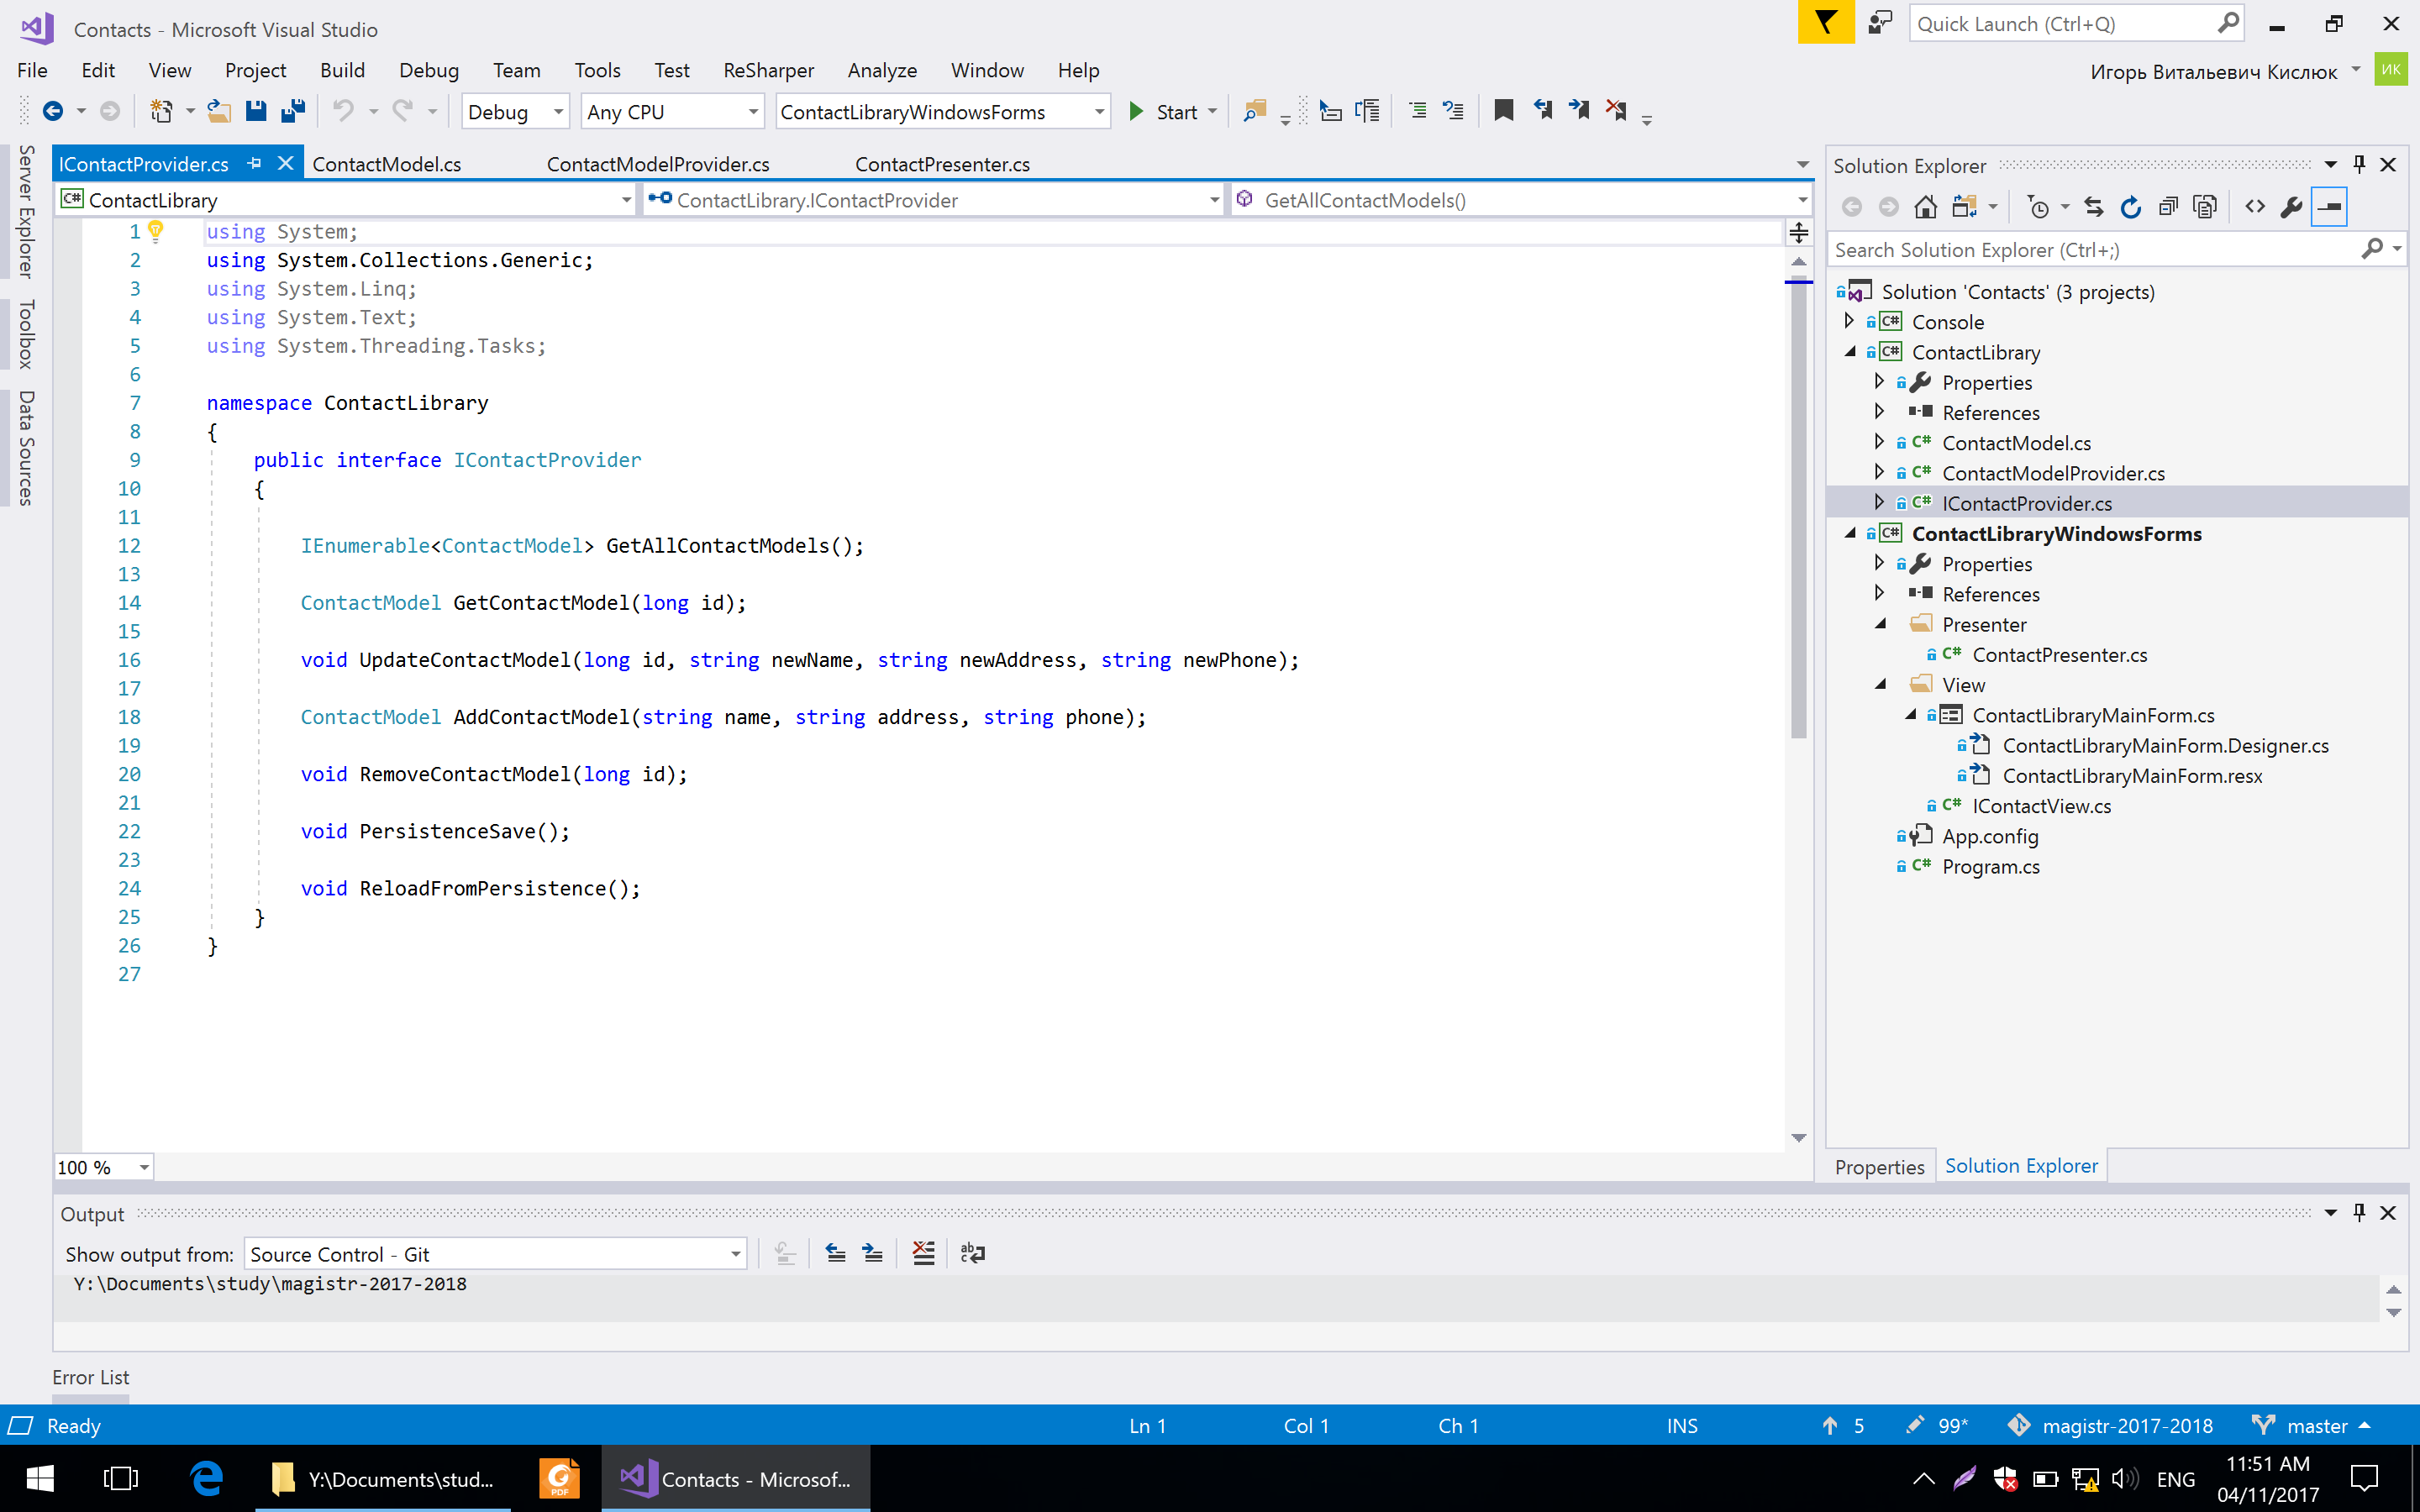
\includegraphics[width=0.8\textwidth]{../screenshots/Screenshot_1}
\caption{Пример интерфейса IContactProvider}
\end{figure}

\item Необходимо реализовать сущность Presenter, которая отвечает за взаимодействие модели и представления, повышая таким образом их изолированность и способность работать независимо. Сущность Presenter внутри будет взаимодействовать с ContactModelProvider - моделью, и представление окна - формой ContactLibraryMainForm.

\begin{figure}[ht]
\centering
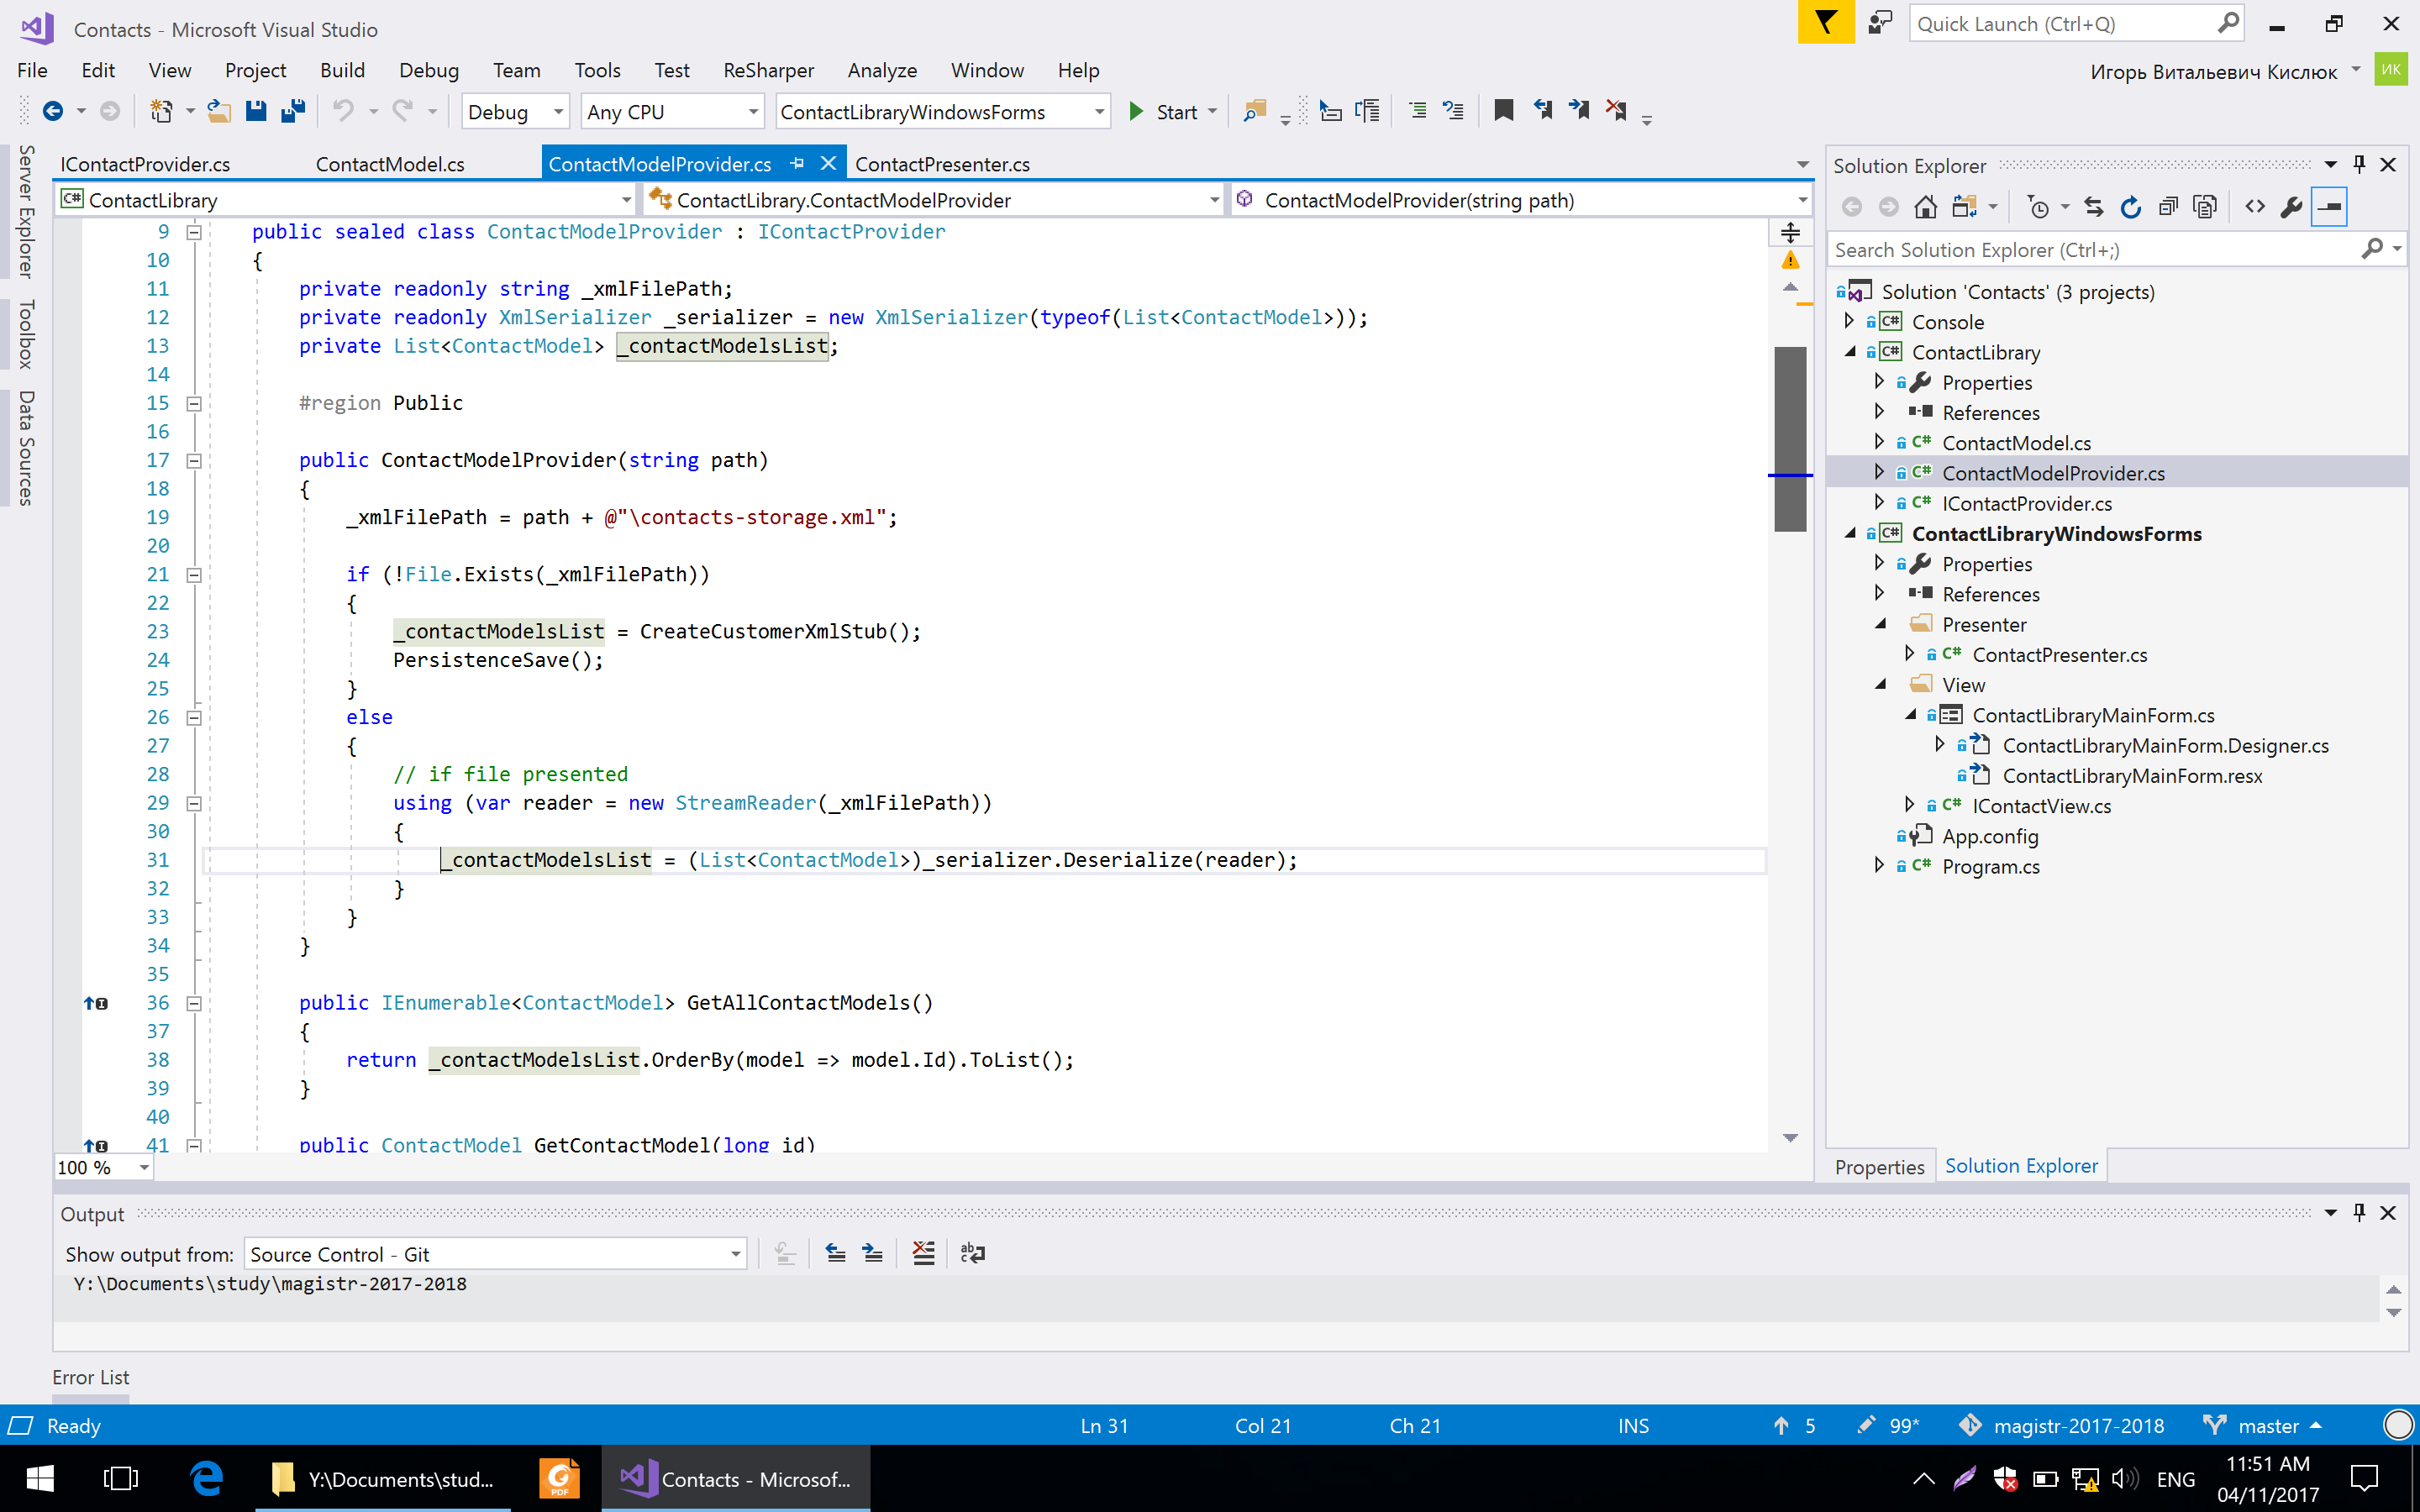
\includegraphics[width=0.8\textwidth]{../screenshots/Screenshot_2}
\caption{Пример реализации сущности Presenter}
\end{figure}

\item Пример работоспособного приложения показан на рисунке~\ref{working-app}.

\begin{figure}[ht]
\centering
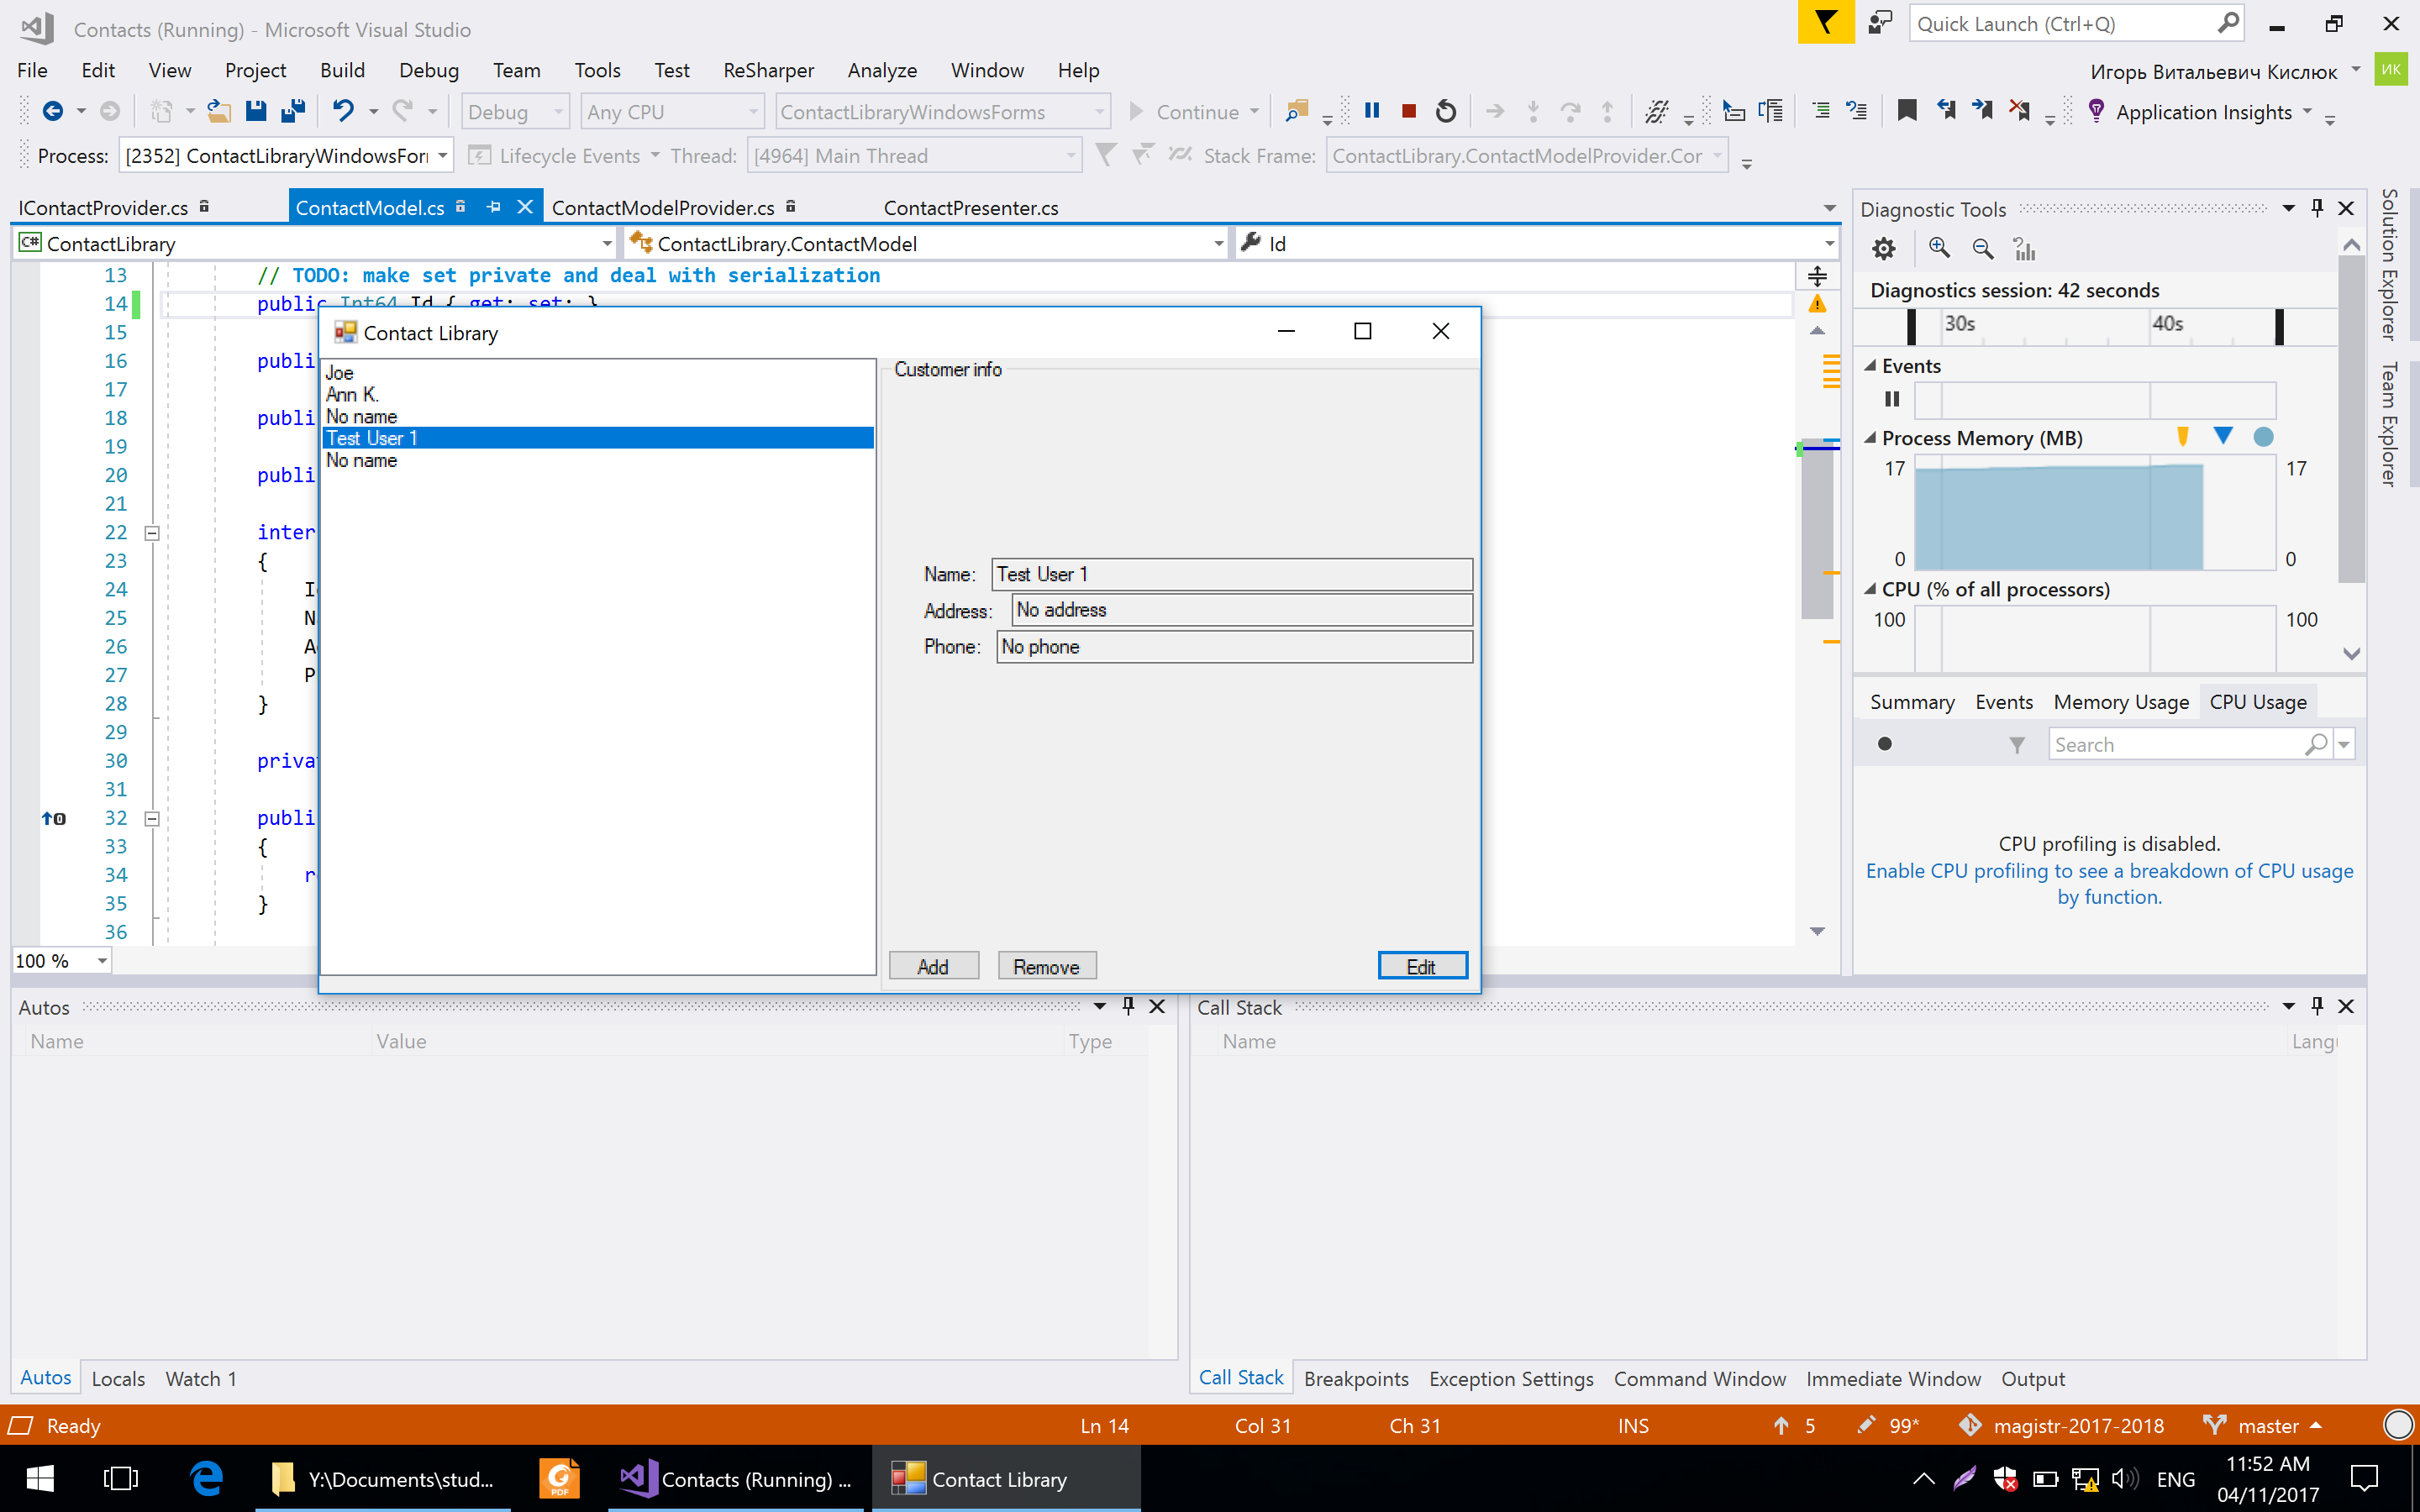
\includegraphics[width=0.8\textwidth]{../screenshots/Screenshot_3}
\caption{Пример использования приложения}
\label{working-app}
\end{figure}

\end{enumerate}

\clearpage

\textbf{Вывод}: таким образом было разработано приложение, которое реализует шаблон MVC, с целью упрощения взаимодействия между различными компонентами. Вид отделен от модели с помощью сущности Presenter, что значительно повышает модульность разработанного приложения.

\end{document}

